% ----------------------------------------------------------
\chapter{Introdução}
% ----------------------------------------------------------

 O conceito de armadura é tão antigo quanto se possa imaginar. As armaduras tem acompanhado o ser humano através dos tempos. Sempre com o mesmo objetivo final, que é proteger recursos valiosos. Muitas vezes este recurso trata-se da própria vida de quem está sendo protegido pela armadura. Paul Hazell fala em seu livro, Armour Materials, Theory and Design, \cite{Hazell}, sobre o que chama de cebola da sobrevivência. Esta é uma analogia para as varias camadas da proteção, ver figura \ref{fig:0.1}.\\
 
 \begin{figure}[h]
 	\caption{Cebola da sobrevivência destacando a direita as camadas abordadas pelo trabalho.}
 	\centering
 	
\includegraphics{images/cebola_sobrevive}
 	\label{fig:0.1}
 	\fonte{\cite{Hazell} traduzido pelo autor.}
 \end{figure}
O foco deste trabalho é revisar a fundamentação teórica da ferramenta mais usada para estudar a camada 4, não ser penetrado, que é a simulação computacional de impactos balísticos. Há certa interação entre não ser penetrado e não ser adquirido. Inicialmente parece enigmático o conceito de não ser adquirido, porém ele nada mais é do que a habilidade de poder escapar da mira humana ou de qualquer sistema de referenciação do projétil. Sendo assim quando se trata de veículos a velocidade é um dos maiores potencializadores da capacidade de não ser adquirido. \\

Um exemplo para a interação citada anteriormente pode ser dado usando veículos com motores a combustão interna. Os tanques são os veículos militares terrestres mais famosos na cultura popular. Em geral, quando comparados a outros veículos terrestres, os tanques tem o balanço desviado para a camada 4, não ser penetrado. Para cumprir sua função o tanque deve carregar munições e armas que quando somados possuem peso significativamente alto. Além disso é normal que o tanque tenha que assumir uma posição de apoio, logo deve permanecer em uma região específica. Somando as características e funções deste veículo, é natural que se construa um veículo com placas de metal espessas que suportem projeteis de energia cinética considerável. Tal construção gera um desequilíbrio em favor do tanque não ser penetrado, em detrimento dele não ser adquirido.\\ 

\begin{figure}[h]
	\caption{\label{fig:0.2} Veículo M1-Abrams}
	\centering
	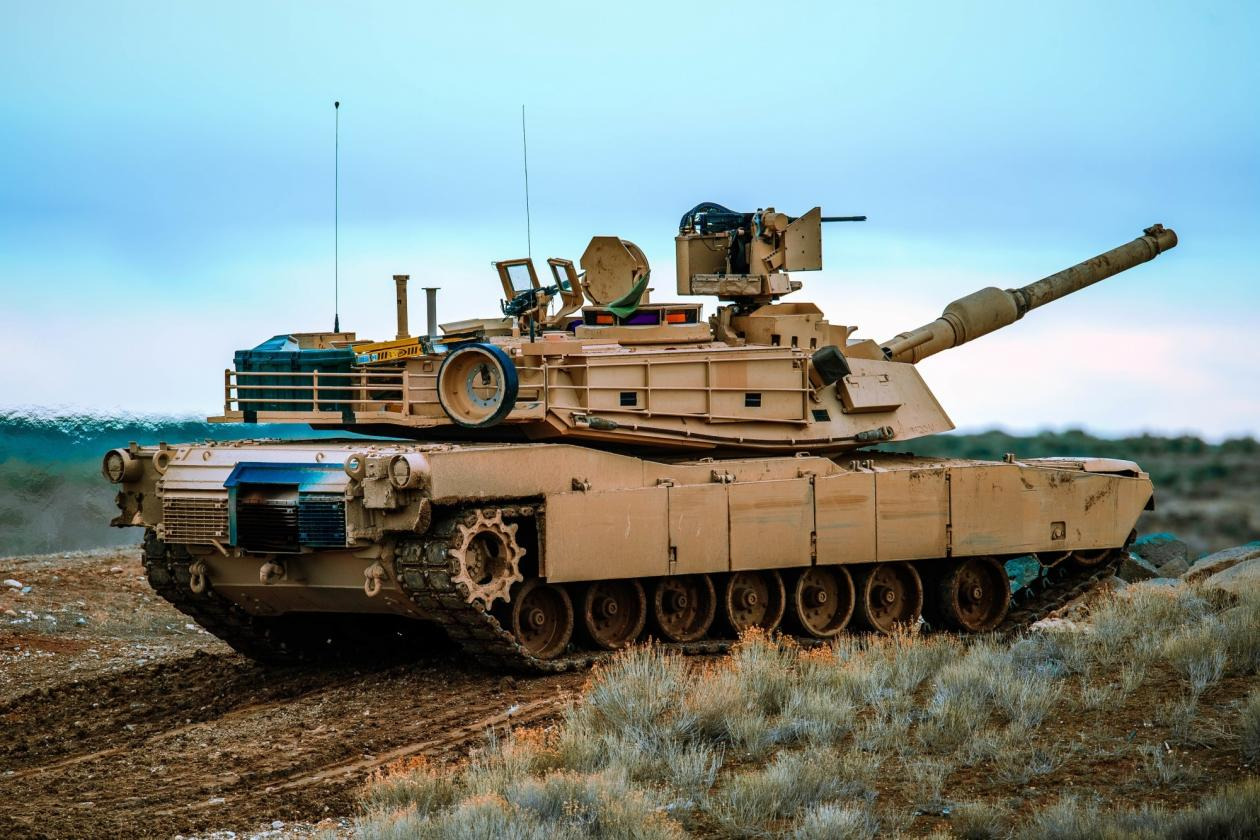
\includegraphics[width=0.7\linewidth]{images/m1-abrams}
	\fonte{https://nationalinterest.org/blog/buzz/us-armys-legendary-m1-abrams-tank-rip-or-ready-war-77621}
\end{figure}

 Do outro lado do espectro estão os veículos mais leves com tarefas variadas. Exemplo disso é o VBMT-LSR do exército brasileiro. Este apresenta desequilíbrio em favor de não ser adquirido, de tal forma que projéteis pesados podem facilmente penetrar sua blindagem. A velocidade e agilidade deste tipo de veículo, tendo um tanque como padrão, aumenta a dificuldade de aquisição. O fato de ter maior dificuldade de aquisição não livra o veículo de ser atingido facilmente por projeteis guiados por sistemas de posicionamento avançados. A motivação da agilidade e rapidez dos veículos leves é o cumprimento de suas funções estratégicas, porém o veículo usa este recurso para sobreviver. \\
 \begin{figure}[h]
 	\caption{\label{fig:0.3} Veículo VBMT-LSR, classificado como veículo leve multitarefa.}
 	\centering
 	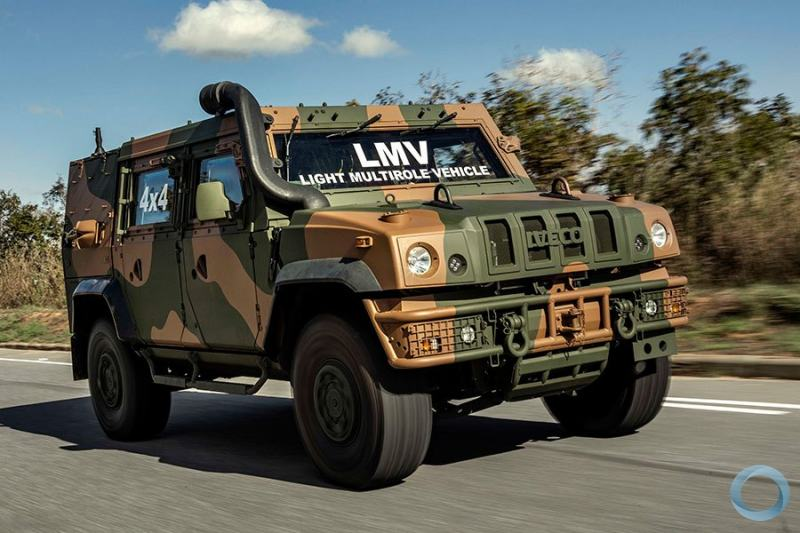
\includegraphics[width=0.7\linewidth]{images/lmv}
 	\fonte{http://www.defesanet.com.br/guarani/noticia/34800/VBMT-LSR---Exercito-Brasileiro-oficializa-a-compra-da-LMV--com-a-IVECO-Veiculos-de-Defesa-/}
 \end{figure} 
\vspace{10mm}

O exemplo mostra o balanço de forma reduzida, dado que existem relações complexas entre as camadas da sobrevivência. Em geral há forte envolvimento da massa do sistema na distribuição de quais camadas são ou não privilegiadas. Normalmente o aumento da capacidade de absorver impacto se dá por meio da inserção de placas massivas, diminuindo a mobilidade do sistema. Este trabalho tem foco nos veículos leves e coletes pessoais, portanto apenas projeteis com velocidade abaixo de $ 2000 m/s$ serão considerados. \\

Para desenvolver este tipo de proteção é necessário entender como ela se comportará face aos impactos que irá sofrer. É possível fazer todo o estudo de comportamento e de possíveis melhorias usando apenas experimentação, porém isto não a melhor opção em relação aos valores investidos. Um caminho viável para tal é usar simulações computacionais aliadas à experimentação. \\

As bases teóricas para a simulação computacional de um evento balístico são o foco desta revisão. A definição das deformações finitesimais e das leis básicas do equilíbrio termomecânico são retiradas da mecânica do contínuo. Então a técnica mais usada para a solução destes problemas será vista, que é a de elementos finitos. Logo após a revisão do método dos elementos finitos os modelos constitutivos serão apresentados dentro do contexto da plasticidade computacional. Por fim a mecânica da penetração será visitada, com foco nos pontos mais importantes para armaduras leves.
 


% ----------------------------------------------------------
\section{Objetivos}
% ----------------------------------------------------------

% ----------------------------------------------------------
\subsection{Objetivo Geral}
% ----------------------------------------------------------

Revisar a fundamentação teórica das áreas de maior influência na simulação computacional de um evento de impacto balístico.

% ----------------------------------------------------------
\subsection{Objetivos Específicos}
% ----------------------------------------------------------

\begin{itemize}
    \item Revisar os fundamentos mecânica do contínuo com foco na descrição de deformações finitesimais e nas leis de equilíbrio.
    \item Revisar os fundamentos do método dos elementos finitos com foco em sistemas dinâmicos.
    \item Revisar os fundamentos da plasticidade computacional e apresentar os modelos mais usados quando altas taxas de deformação estão presentes.
    \item Revisar o processo de penetração de projéteis com velocidades inferiores a $2000 m/s$
\end{itemize}